\section{The Decomposition: Perception, Recognition, Knowledge, and Intelligence}

\subsection{Overview}

Before intelligence can be analyzed dynamically, it must be separated from neighboring layers that are often conflated with it. This section distinguishes four layers:

\begin{enumerate}
\item perception,
\item recognition,
\item knowledge,
\item intelligence.
\end{enumerate}

The distinction is structural rather than psychological. It does not assert that these layers occur separately in an organism or machine. It states that they perform different structural roles. Confusing them produces many of the classical difficulties in theories of intelligence.

\subsection{Perception}

Perception is the layer at which availability first appears. Something becomes available to a system as a differentiated input. Perception does not yet require classification, mapping, knowledge, or inference. It requires only that a difference be registered as accessible to the system.

In this sense, perception is a precursor layer. It forms inputs, but it does not by itself determine what those inputs are, how they relate to prior states, or how they should be used.

\subsection{Recognition}

Recognition is the layer at which available inputs become mappable. A perceived difference is related to a schema, pattern, category, or prior configuration. Recognition therefore adds relational structure to perception.

Recognition remains a precursor layer because mapping is not yet stabilization. A recognized pattern can still be unstable, ambiguous, revisable, or false. Recognition allows a system to say that something is like something else, but it does not by itself produce a stable stopping structure.

\subsection{Knowledge}

Knowledge is a stopping structure. It is a state that can be stored, cited, transmitted, and treated as established within a given window. Knowledge is not identical with intelligence. It is one of the products that intelligence can generate.

The defining feature of knowledge is stability. A knowledge state can function as a reference point, a premise, or a stored result. It can be reused because it has stopped, at least locally and provisionally.

This is why knowledge is vulnerable to Gettier-type problems. A stopping structure can be true, justified, and believed while still failing to carry the dynamic property that intelligence requires. A stopped result cannot guarantee the motion that produced it.

\subsection{Intelligence}

Intelligence is not a stopping structure. It is ongoing motion across the previous layers. It forms inputs, maps them, stabilizes temporary stopping structures, revises those structures, and reopens them when new relations appear.

The essential property of intelligence is revisability. Intelligence operates by generating and traversing stopping structures without becoming one of them. It is not stored in perception, recognition, or knowledge. It moves through them.

\begin{quote}
Knowledge is a stopping structure.\\
Intelligence is the dynamics that continually produces, revises, and traverses such stopping structures.
\end{quote}

\subsection{Why the distinction matters}

If knowledge and intelligence are conflated, then one expects a stored proposition to carry a dynamical property. This is the structural source of the Gettier-type confusion discussed in \S{}6.

If recognition and intelligence are conflated, then pattern matching is mistaken for ongoing adaptive motion. If perception and intelligence are conflated, then mere availability is mistaken for structural transformation.

The decomposition therefore prepares the rest of the paper. The three axioms in \S{}3 describe the minimal conditions for the fourth layer, not for perception, recognition, or knowledge.

\begin{figure}[H]
\centering
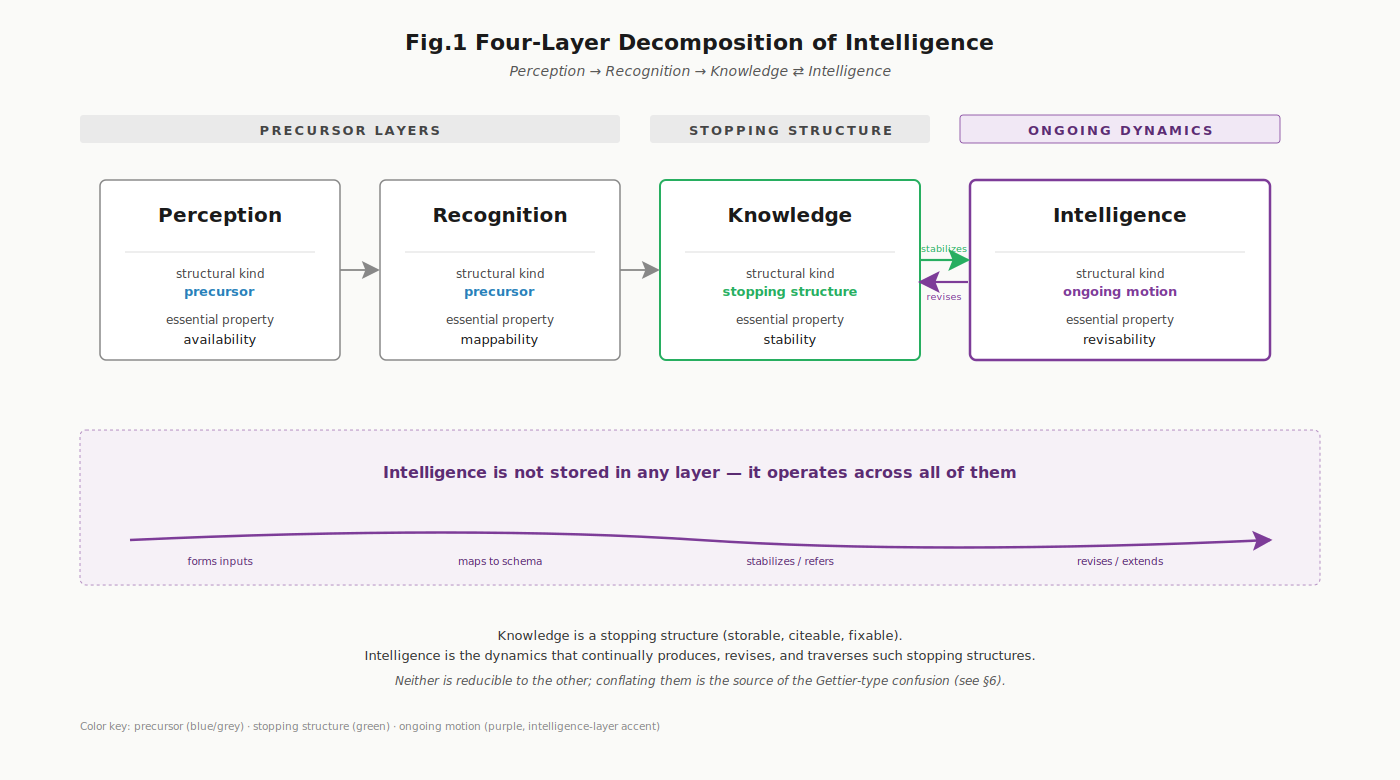
\includegraphics[width=\textwidth]{figures/fig1_four_layer_decomposition.png}
\caption{Four-layer decomposition of intelligence. Perception and recognition are precursor layers, knowledge is a stopping structure, and intelligence is ongoing revisable motion across all of them.}
\label{fig:intelligence_part1_1}
\end{figure}
